\documentclass[a4paper]{article}
\usepackage[a4paper, left=15mm, right=15mm, top=15mm, bottom=15mm]{geometry}
\usepackage[utf8]{inputenc}
\usepackage{indentfirst}
\usepackage{amsmath}
\usepackage{amssymb}
\usepackage{graphicx}
\usepackage{float}
\usepackage{amsthm}

\DeclareMathOperator*{\argmin}{arg\,min}

\newcommand{\F}{\mathcal{F}}
\newcommand{\R}{\mathbb{R}}
\newcommand{\conv}{\mbox{conv}\,}

\renewcommand{\baselinestretch}{1.3}

\theoremstyle{definition}
\newtheorem{definition}{Definition}[section]

\title{On the feasibility for the system of quadratic equations\\MATLAB Library}
\date{}
\author{Anatoly Dymarsky, Elena Gryazina, Boris Polyak, Sergei Volodin}

\begin{document}
\maketitle
\section{Notations}
The goal of the project is to solve a number of tasks for quadratic maps, which are
\begin{enumerate}
\item (Real case) The map $f\colon \mathbb{R}^n\to\mathbb{R}^m$ s.t. $$f_i(x)=x^TA_ix+2b_i^Tx,\, A_i=A_i^T$$
\item (Complex case) The map $f\colon \mathbb{C}^n\to\mathbb{R}^m$ s.t. $$f_i(x)=x^*A_ix+b_i^*x+x^*b_i,\, A_i=A_i^*$$
Where $\cdot^*$ is Hermitian conjugate.
\end{enumerate}

From this point on, $X$ denotes $\mathbb{R}^n$ for real case or $\mathbb{C}^n$ for complex case.

We use the following notations:
\theoremstyle{definition}
\begin{definition} For scalars, vectors, tuples of vectors or tuples of matrices $A=(A_1,...,A_n)\in X^n$ and $B=(B_1,...,B_n)$ the dot product is defined as following: $$A\cdot B=\sum\limits_{i=1}^nA_i\cdot B_i$$
For example, for a vector $c\in \mathbb{R}^n$ and a tuple of matrices $A=(A_1,...,A_n)$, $A_i\colon m\times m$ the expression $c\cdot A=\sum\limits_{i=1}^nc_iA_i$ is a matrix $c\cdot A\colon m\times m$.
\end{definition}
\begin{definition} The image of $f$ is denoted as $F$:
	$$F=f(X)$$
\end{definition}
\begin{definition} The convex hull of $F$ is denoted as $G$:
	$$G=\conv F$$
\end{definition}
\begin{definition} The boundary points of $F$ (or $G$) touched by a supporting hyperplane with the normal vector $c\in\mathbb{R}^m$:
	$$\partial F_c=\partial G_c=\argmin\limits_{y\in F}(c\cdot y)$$
\end{definition}
\section{Functions}
The library consists of a number of functions defined in separate .m files. Input format for the map is the following: 

\begin{itemize}
\item The number $A(i, j, k)$ denotes $i$'th row and $j$'th column of the matrix $A_k$
\item The number $b(i, j)$ denotes $i$'th element of the vector $b_j\in\mathbb{R}^m$
\end{itemize}

\begin{enumerate}
\item {\bf Feasibility membership oracle.} Given:
\begin{itemize}
\item The map $f$ as matrices $A$ and vectors $b$
\item A point $y\in\mathbb{R}^m$.
\end{itemize}
{\bf Determine:} if $y\in F$

\begin{figure}[H]
	\centering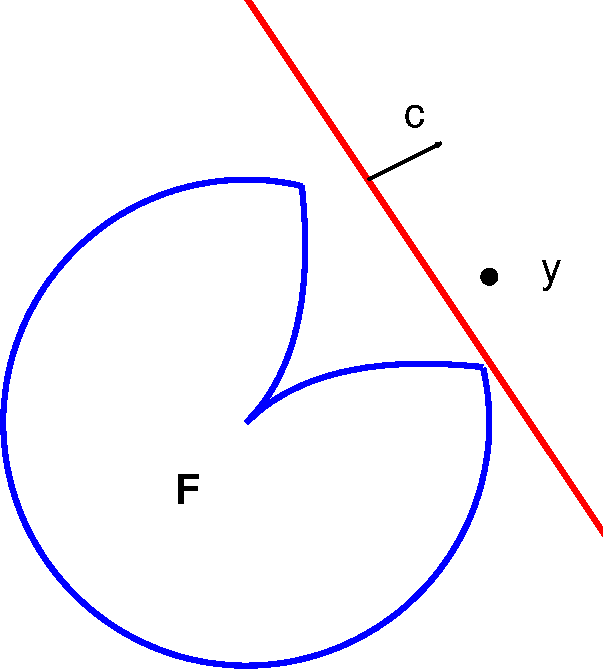
\includegraphics[width=100pt]{infeasibility_oracle}
	\caption{Infeasibility oracle: hyperplane $c$ separates the point $y^0$ from the image $F$}
\end{figure}

\begin{verbatim}
is_infeasible = infeasibility_oracle(A, b, y)
\end{verbatim}

This function tries to separate the point $y$ from the convex hull $G$ with a hyperplane. See Theorem 3.2 from the article.

{\bf Return value:} $1$ means that the separation was successful and the point $y\notin G$. This implies $y\notin F$. On the contrary, $0$ means that the feasibility is uncertain.

\item {\bf Boundary oracle.} Given:
\begin{itemize}
	\item The map $f$ as matrices $A$ and vectors $b$
	\item A point $y\in G$
	\item A direction $d\in\R^m$
\end{itemize}
The following two tasks are considered:
\begin{enumerate}
\item {\bf Find:} distance to the boundary from a given point inside $G$.

\begin{figure}[H]
	\centering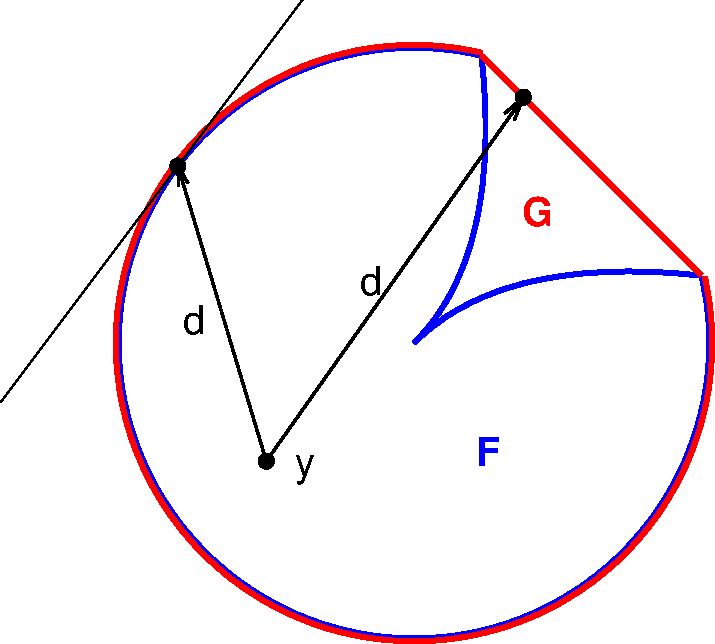
\includegraphics[width=100pt]{boundary_oracle}
	\caption{Boundary oracle: distance from $y$ to the boundary $\partial G$ in direction $d$}
\end{figure}

\begin{verbatim}
[t, is_in_F] = boundary_oracle(A, b, y, d)
\end{verbatim}

This function finds the point $y+td$ on the boundary $\partial G$ with the largest $t$:
$$t = \sup\{\tau\big| y+\tau d\in G\}$$
{\bf Return value:}
\begin{itemize}
	\item $t$ is the largest step in direction $d$ such that $y+td$ is still in $G$.
	\item is\_in\_F is a binary variable indicating if the resulting point $y+td$ belongs to $F$: it is 1 if it is true or 0 if the result is uncertain
\end{itemize}

{\bf Exception:} if optimization task failed, in particular, if $y\notin G$ or the normal vector does not exist at that point.

\item {\bf Find:} the normal vector $c$ at the boundary point $y+td$.

\begin{figure}[H]
	\centering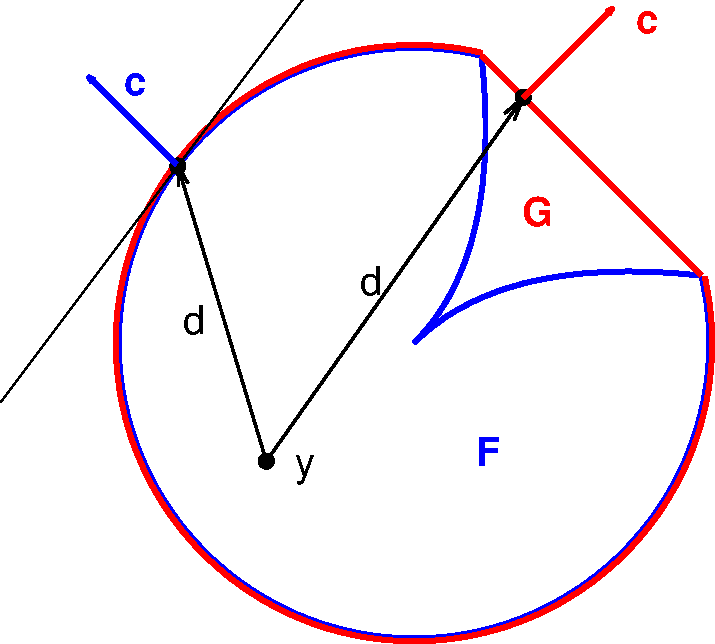
\includegraphics[width=100pt]{get_c_from_d}
	\caption{Boundary oracle: normal vector $c$ at boundary point $y+td$}
\end{figure}

\begin{verbatim}
c = get_c_from_d(A, b, y, d)
\end{verbatim}

This function obtains the normal vector $c$ at the boundary point $y+td$ using dual problem (5) from the article.

{\bf Return value:} the normal vector $c$ s.t. $y+td\in\partial G_c$

{\bf Exception:} if optimization task failed, in particular, if $y\notin G$ or the normal vector does not exist at this point.
\end{enumerate}

\item {\bf Nonconvexity certificate.} Given:
\begin{itemize}
	\item The map $f$ as matrices $A$ and vectors $b$
	\item A point $y\in F$
	\item Number of iterations $k$
\end{itemize}
The following two tasks are considered:
\begin{enumerate}
	\item {\bf Find:} a vector $c$ such that $\partial F_c$ is nonconvex.
	
	\begin{verbatim}
	c = get_c_minus(A, b, y, k)
	\end{verbatim}
	This function is generating at most $k$ random directions $d$ and checks if the intersection of the boundary $\partial G_c$ with a hyperplane with normal vector $c$ at the boundary point $y+td$ is nonconvex.

	{\bf Return value:}  $c$ s.t. $\partial F_c$ is nonconvex
	
	{\bf Exception:} if $c$ was not found in $k$ iterations
	
	\item {\bf Determine:} if $F$ is nonconvex.
	
	\begin{verbatim}
	is_nonconvex = nonconvexity_certificate(A, b, y, k)
	\end{verbatim}
	
	This function checks if the image is nonconvex via obtaining $c\in C_-$. If $c$ was found in $k$ iterations, the image $F$ is guaranteed to be nonconvex, Otherwise the result is uncertain
	
	{\bf Return value:} $1$ if $F$ is nonconvex, $0$ if result is uncertain
\end{enumerate}

\item {\bf Positive-definite $c\cdot A$.} Given:
\begin{itemize}
	\item The map $f$ as matrices $A$ and vectors $b$
	\item The initial normal vector $p$
\end{itemize}
The following three tasks are considered:
\begin{enumerate}
	\item {\bf Find:} vector $c_+$, s.t. $c_+\cdot A\succ 0$
	
	\begin{verbatim}
	c_plus = get_c_plus(A, k)
	\end{verbatim}
	
	This function generates a random vector $p$ and then finds $c_+$ nearest to it. Function generates at most $k$ vectors $p$.
	
	{\bf Return value:} $c_+$ s.t. $c_+\cdot A\succeq 0$
	
	{\bf Exception:} if $c_+$ was not found
	
	\item {\bf Find:} $c_+$, s.t. the convex cut is maximal.
	
	\begin{verbatim}
	c_plus = get_max_c_plus(A)
	\end{verbatim}
	
	This function returns the ''best'' vector $c$ s.t. $c\cdot A\succeq 0$ and $\lambda_{\min}(c\cdot A)\to\max$. The spectrum of the resulting matrix $c_+\cdot A$ is separated from $0$ the most. This is a heuristic trying to achieve maximal value of $z_{\max}$ in this direction.
	
	{\bf Return value:} $c_+$ s.t. $c_+\cdot A\succeq 0$
	
	{\bf Exception:} if $c_+$ was not found
	
	\item {\bf Find:} $c_+$ close to given arbitrary $p$.
	
	\begin{verbatim}
	c_plus = get_near_c_plus(A, p, gamma);
	\end{verbatim}
	
	This function finds the nearest to $p$ vector $c_+$ such that $c_+\cdot A\succeq 0$ heuristically from the neighbourhood of $p$.
	
	{\bf Return value:}  $c_+$ s.t. $c_+\cdot A\succeq 0$
	
	{\bf Exception:} if $c_+$ was not found
	
\end{enumerate}

\item {\bf Convex subpart.} Given:
\begin{itemize}
	\item The map $f$ as matrices $A$ and vectors $b$
	\item The number $z_{\max}^{\mbox{\small guess}}$
	\item Number of iterations $k$
	\item Vector $c_+$ s.t. $c_+\cdot A\succeq 0$
\end{itemize}

{\bf Find:} maximal convex cut of $F$.

\begin{figure}[H]
	\centering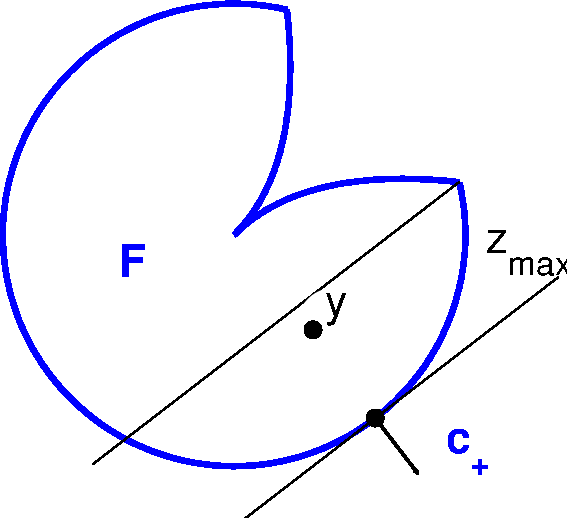
\includegraphics[width=100pt]{get_z_max}
	\caption{Convex subpart: maximal value of $z_{\max}$ such that a cut with a hyperplane $c_+$ is still convex}
\end{figure}

\begin{verbatim}
z_max = get_z_max(A, b, c_plus, z_max_guess, k)
\end{verbatim}

This function returns the maximal value $z_{\max}$ such that the cut in the direction of $c_+$ of size $z_{\max}$ is still convex. This procedure is a heuristic (convexity of maximality is not guaranteed).

The value $z_{\max}^{\mbox{\small guess}}$ generates a point $y=y_0-z_{\max}^{\mbox{\small guess}}c_+$, where $y_0$ is the touching point of hyperplane $c_+$ which is used for the nonconvexity certificate.

{\bf Return value:} Maximal value $z_{\max}$ or Inf if no nonconvexities were found

{\bf Exception:} None
\end{enumerate}
\end{document}
